\documentclass[tikz,border=6pt]{standalone}
\usepackage{amsmath,amssymb}
\definecolor{cA}{RGB}{31,94,165}\definecolor{cB}{RGB}{214,96,33}
\tikzset{
  t/.style={circle,inner sep=0pt,minimum size=8.5pt,ball color=cA!85,draw=cA!60!black,line width=0.3pt},
  b/.style={circle,inner sep=0pt,minimum size=8.5pt,ball color=cB!90,draw=cB!60!black,line width=0.3pt},
  e/.style={line width=0.9pt,black!60},
  r/.style={line width=0.9pt,black!40},
  lab/.style={font=\scriptsize,inner sep=1pt}}
\pgfdeclarelayer{bg}\pgfsetlayers{bg,main}
\begin{document}
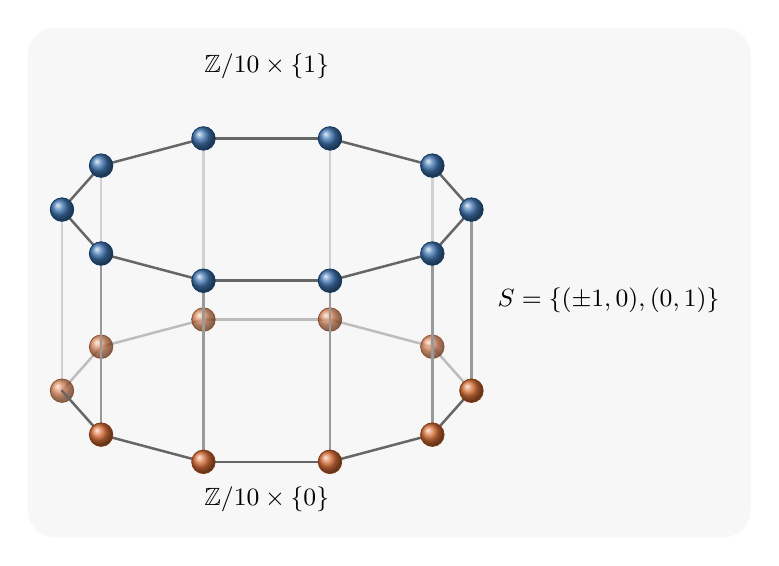
\begin{tikzpicture}[x={(2.6cm,0cm)},y={(0cm,0.95cm)},z={(0cm,2.3cm)},line cap=round]
\draw[e,opacity=0.4] (1.0000,0.0000,0.0000) -- (0.8090,0.5878,0.0000);
\draw[e,opacity=0.4] (0.8090,0.5878,0.0000) -- (0.3090,0.9511,0.0000);
\draw[e,opacity=0.4] (0.3090,0.9511,0.0000) -- (-0.3090,0.9511,0.0000);
\draw[e,opacity=0.4] (-0.3090,0.9511,0.0000) -- (-0.8090,0.5878,0.0000);
\draw[e,opacity=0.4] (-0.8090,0.5878,0.0000) -- (-1.0000,0.0000,0.0000);
\draw[r,opacity=0.4] (0.8090,0.5878,0.0000) -- (0.8090,0.5878,1.0000);
\draw[r,opacity=0.4] (0.3090,0.9511,0.0000) -- (0.3090,0.9511,1.0000);
\draw[r,opacity=0.4] (-0.3090,0.9511,0.0000) -- (-0.3090,0.9511,1.0000);
\draw[r,opacity=0.4] (-0.8090,0.5878,0.0000) -- (-0.8090,0.5878,1.0000);
\draw[r,opacity=0.4] (-1.0000,0.0000,0.0000) -- (-1.0000,0.0000,1.0000);
\node[b,opacity=0.75] at (0.8090,0.5878,0.0000) {};
\node[b,opacity=0.75] at (0.3090,0.9511,0.0000) {};
\node[b,opacity=0.75] at (-0.3090,0.9511,0.0000) {};
\node[b,opacity=0.75] at (-0.8090,0.5878,0.0000) {};
\node[b,opacity=0.75] at (-1.0000,0.0000,0.0000) {};
\draw[e] (0.3090,-0.9511,1.0000) -- (0.8090,-0.5878,1.0000);
\draw[e] (0.8090,-0.5878,1.0000) -- (1.0000,0.0000,1.0000);
\draw[e] (1.0000,0.0000,1.0000) -- (0.8090,0.5878,1.0000);
\draw[e] (0.8090,0.5878,1.0000) -- (0.3090,0.9511,1.0000);
\draw[e] (0.3090,0.9511,1.0000) -- (-0.3090,0.9511,1.0000);
\draw[e] (-0.3090,0.9511,1.0000) -- (-0.8090,0.5878,1.0000);
\draw[e] (-0.8090,0.5878,1.0000) -- (-1.0000,0.0000,1.0000);
\draw[e] (-1.0000,0.0000,1.0000) -- (-0.8090,-0.5878,1.0000);
\draw[e] (-0.8090,-0.5878,1.0000) -- (-0.3090,-0.9511,1.0000);
\draw[e] (-0.3090,-0.9511,1.0000) -- (0.3090,-0.9511,1.0000);
\draw[e] (0.3090,-0.9511,0.0000) -- (0.8090,-0.5878,0.0000);
\draw[e] (0.8090,-0.5878,0.0000) -- (1.0000,0.0000,0.0000);
\draw[e] (-1.0000,0.0000,0.0000) -- (-0.8090,-0.5878,0.0000);
\draw[e] (-0.8090,-0.5878,0.0000) -- (-0.3090,-0.9511,0.0000);
\draw[e] (-0.3090,-0.9511,0.0000) -- (0.3090,-0.9511,0.0000);
\draw[r] (0.3090,-0.9511,0.0000) -- (0.3090,-0.9511,1.0000);
\draw[r] (0.8090,-0.5878,0.0000) -- (0.8090,-0.5878,1.0000);
\draw[r] (1.0000,0.0000,0.0000) -- (1.0000,0.0000,1.0000);
\draw[r] (-0.8090,-0.5878,0.0000) -- (-0.8090,-0.5878,1.0000);
\draw[r] (-0.3090,-0.9511,0.0000) -- (-0.3090,-0.9511,1.0000);
\node[b] at (0.3090,-0.9511,0.0000) {};
\node[b] at (0.8090,-0.5878,0.0000) {};
\node[b] at (1.0000,0.0000,0.0000) {};
\node[b] at (-0.8090,-0.5878,0.0000) {};
\node[b] at (-0.3090,-0.9511,0.0000) {};
\node[t] at (0.3090,-0.9511,1.0000) {};
\node[t] at (0.8090,-0.5878,1.0000) {};
\node[t] at (1.0000,0.0000,1.0000) {};
\node[t] at (0.8090,0.5878,1.0000) {};
\node[t] at (0.3090,0.9511,1.0000) {};
\node[t] at (-0.3090,0.9511,1.0000) {};
\node[t] at (-0.8090,0.5878,1.0000) {};
\node[t] at (-1.0000,0.0000,1.0000) {};
\node[t] at (-0.8090,-0.5878,1.0000) {};
\node[t] at (-0.3090,-0.9511,1.0000) {};
\node[font=\small,anchor=west] at (1.08,0,0.5) {$S=\{(\pm1,0),(0,1)\}$};
\node[font=\small] at (0,-1.45,0) {$\mathbb{Z}/10\times\{0\}$};
\node[font=\small] at (0,1.0,1.38) {$\mathbb{Z}/10\times\{1\}$};
\begin{pgfonlayer}{bg}
\fill[black!3,rounded corners=10pt] ([shift={(-8pt,-6pt)}]current bounding box.south west) rectangle ([shift={(8pt,6pt)}]current bounding box.north east);
\end{pgfonlayer}
\end{tikzpicture}\end{document}